% Provenance (never printed): see sources/outline_sources.md (Year 3:
% moments of inertia and gravity fields; impact cratering and crater dating;
% volcanism and tectonics on Mars, Venus, Io and the icy moons).
% Brief: sources/book5/BRIEFS.md, ch. 26. Curves from figdata/bachelor-3/
% two_layer_planet.py (two-layer interiors of the Earth, Mars, the Moon and
% Mercury from mean density and moment of inertia) and crater_sfd.py
% (the Ivanov production function and the Hartmann-Neukum chronology of
% Mars from the Craterstats configuration, the lunar chronology of Neukum,
% Hartmann's equilibrium density, and two invented Martian plains whose
% counts are drawn once from a Poisson law). Exercise and problem values in
% the Book 5 scratch calculator calc/ch26.py. Plains A and B are invented.
\chapter{بواطن الكواكب وأسطحها}\label{ch:b3:planetary-interiors-surfaces}

يبدو للقمر عند رصده بالمنظار نوعان من السطح. والمرتفعات الفاتحة
مغطّاة بالفوهات، فوهةٌ فوق فوهة: فقد أُشبعت
بالفوهات الكبيرة بفعل قصفٍ شديد انتهى منذ نحو 3.8 مليار
سنة. أمّا السهول المظلمة، وهي سهول ملأتها الحمم بين 4.2 و1.2 مليار
سنة مضت، فتحمل فوهاتٍ أقلّ بكثير. وقد جلبت بعثتا أبولو ولونا
صخورًا من النوعين، فحوّلت أعمارها الإشعاعية
كثافةَ الفوهات على سطحٍ ما إلى ساعة. وتؤرّخ هذه الساعة الآن
السهول على المريخ وعطارد والأقمار الجليدية، التي لم تُجلب منها بعدُ أيّ صخرة
إلى الأرض. ويقرأ هذا الفصل بواطن الكواكب من خلال
جاذبيتها ودورانها ومدّها، ثم أسطحها في فوهاتها،
وبراكينها وصدوعها.
% ledger: french:highlands, nasa:moon-core, marchi:neukum

\begin{recall}
يرد عامل عزم القصور الذاتي $C = I/MR^2$، ونموذج الطبقتين لكوكبٍ
يُبنى منه ومن الكثافة المتوسطة، والكواكب الأرضية والعملاقة، في مجلد
السنة الأولى، في فصله عن علم الكواكب المقارن؛ وأعمدة الوشاح
والأقاليم البركانية الكبرى، في فصله عن
البقع الساخنة. ويرد التمايز الكوكبي والنيازك في مجلد السنة الثانية،
في فصله عن نشأة الكواكب. ويرد \omterm{def:b3:gravity-geodesy:j2}{معامل الشكل الديناميكي} $J_2$،
\omterm{thm:b3:gravity-geodesy:maccullagh}{وصيغة ماكولا} \omterm{def:b3:gravity-geodesy:flexure}{وانثناء الغلاف الصخري} في هذا المجلد، في فصله عن
الجاذبية والجيوديسيا؛ \omterm{def:b3:mantle-convection:rayleigh}{وعدد رايلي} في فصله عن الحمل في الوشاح.
ويرد المدّ وقوانين كبلر ومعاملات المرونة في كتب الفيزياء؛
وتوزيع بواسون في
كتب الرياضيات.
\end{recall}

\section{البواطن من الجاذبية والدوران والمدّ}\label{sec:b3:planetary-interiors-surfaces:interiors}

تُعطي كتلةُ الكوكب، المستمدّة من مدار قمرٍ أو مركبةٍ فضائية، كثافتَه المتوسطة؛
ويُعطي التقدّمُ المحوري للكوكب و$J_2$ عزمَ قصوره الذاتي.
وتحوّل قضيةُ الطبقتين الواردة في مجلد السنة الأولى الرقمين إلى لبّ،
لكن بعد اختيار كثافة الوشاح فحسب، إذ لا يمكن لقياسين أن يعيّنا
ثلاثة مجهولات.

\begin{omfigure}
\centering
\begin{tikzpicture}
\begin{axis}[width=0.78\linewidth, height=0.46\linewidth,
  xmin=3000, xmax=16000, ymin=0, ymax=1,
  xlabel={كثافة اللبّ $\rho_c$ \babelsublr{(\unit{kg.m^{-3}})}},
  ylabel={نصف قطر اللبّ / نصف قطر الكوكب $x$},
  tick label style={font=\scriptsize}, label style={font=\small},
  scaled x ticks=false, xtick={4000,6000,8000,10000,12000,14000,16000},
  xticklabels={4000,6000,8000,10\,000,12\,000,14\,000,16\,000}]
\addplot[thick, omDef] table[x=rho_c, y=x] {figdata/out/bachelor-3-two_layer_planet-curve-Earth.dat};
\addplot[thick, red!70!black] table[x=rho_c, y=x] {figdata/out/bachelor-3-two_layer_planet-curve-Mars.dat};
\addplot[thick, black!60, dashed] table[x=rho_c, y=x] {figdata/out/bachelor-3-two_layer_planet-curve-Moon.dat};
\addplot[thick, orange!80!black] table[x=rho_c, y=x] {figdata/out/bachelor-3-two_layer_planet-curve-Mercury.dat};
\addplot[only marks, mark=*, mark size=2pt, black] table[x=rho_c, y=x] {figdata/out/bachelor-3-two_layer_planet-points.dat};
\node[font=\scriptsize, omDef, anchor=south west] at (axis cs:12600,0.55) {الأرض};
\node[font=\scriptsize, red!70!black, anchor=south west] at (axis cs:6600,0.55) {المريخ};
\node[font=\scriptsize, black!70, anchor=south west] at (axis cs:11000,0.2) {القمر};
\node[font=\scriptsize, orange!80!black, anchor=south west] at (axis cs:7300,0.83) {عطارد};
\end{axis}
\end{tikzpicture}
\par\smallskip{\small النماذج ذات الطبقتين المسموح بها بالكثافة المتوسطة
وعامل عزم القصور الذاتي لأربعة أجرام: يمتدّ كلّ منحنى على كثافات
الوشاح الممكنة، فكلّما كان الوشاح أكثف صغُر اللبّ
وازدادت كثافته. وتشير النقاط إلى أنصاف أقطار اللبّ المقاسة: للأرض من علم الزلازل،
وللمريخ من جهاز قياس الزلازل إنسايت، ولقمر لبٌّ داخلي وقشرة سائلة،
ولعطارد من الحقل الثقالي لمركبة MESSENGER
الفضائية.}\label{fig:b3:planetary-interiors-surfaces:two-layer}
\end{omfigure}
% ledger: planet:Earth.density, planet:Mars.density, planet:Moon.density, planet:Mercury.density, earth:MoI, nasa:mars, nasa:moon, nasa:mercury, data:prem, jpl:insight-interior, nasa:moon-core, agu:mercury-core

يُعطي كلّ كوكب منحنًى لا نقطةً. ففي حالة المريخ، يختار نصف قطر اللبّ
المقاس بجهاز إنسايت، وهو \qty{1830}{km}، وشاحًا كثافته \qty{3460}{kg.m^{-3}}
ولبًّا كثافته \qty{6460}{kg.m^{-3}}. وبالنسبة إلى عطارد، فإنّ اللبّ نصف قطره نحو
\qty{2000}{km} يملأ 82~بالمئة من نصف القطر. ومنحنى القمر
شبه مسطّح، إذ إنّ قيمة $C = 0.394$ قريبة جدًّا من $\tfrac25$ بحيث يتّسع لبّ صغير
من أيّ كثافة، ويُحرّك تغيّرُ $0.001$ في $C$ نصفَ قطر اللبّ
بأكثر من الضعف (انظر \cref{exo:b3:planetary-interiors-surfaces:10}).
ولا تكشف الجاذبية وحدها عن لبّ صغير، أمّا المدّ والموجات الزلزالية فتكشف عنه.
% ledger: jpl:insight-interior, agu:mercury-core, nasa:moon

\begin{definition}[عدد لوف]\label{def:b3:planetary-interiors-surfaces:love-number}
حين يؤثّر جهدٌ مدّيّ من الدرجة~2 في كوكب، يتشوّه الكوكب، فتُضيف كتلتُه
المعاد توزيعها جهدًا خاصًّا بها. ويُعرَّف
\emph{عدد لوف}\index{عدد لوف} $k_2$ بأنّه نسبة الجهد المضاف إلى الجهد المدّي،
كلاهما مأخوذ عند سطح الكوكب.
\end{definition}

يكون للكوكب الصلب $k_2 = 0$؛ أمّا الكوكب المائع ذو الكثافة المنتظمة
فيخضع كليًّا، مع $k_2 = \tfrac32$. وبين الطرفين يقيس العدد مقدارَ
ما يستجيب من الكوكب للتشوّه.

\begin{proposition}[عدد لوف لكرة مرنة منتظمة]\label{prop:b3:planetary-interiors-surfaces:kelvin}
لتكن كرةٌ غير قابلة للانضغاط، كثافتها المنتظمة $\rho$، ونصف قطرها $R$، وجاذبيتها
السطحية $g$ وصلابتها $\mu$، ويكون لها
\[
  k_2 = \frac{3/2}{1 + \dfrac{19\mu}{2\rho g R}} .
\]
\end{proposition}

وتُقبل النتيجة المنسوبة إلى كلفن دون برهان. وتقارن النسبة $\mu/\rho gR$
الصلابةَ المرنة بالثقالة الذاتية التي تسحب الانتفاخَ المدّي
إلى الخلف: فالكواكب الصغيرة صلبة، والكبيرة تخضع. وبالنسبة إلى المريخ، $\rho gR =
\qty{4.97e10}{Pa}$؛ وبصلابة الوشاح العلوي للأرض،
\qty{67}{GPa} عند عمق \qty{80}{km} في نموذج الأرض المرجعي،
فتُعطي الصيغة $k_2 = 0.109$. وقاس تتبّعُ المركبة المدارية مارس غلوبال سيرفيور
المدّ الشمسي للمريخ: $k_2 = 0.153 \pm 0.017$، وهي أكبر من أن تُعزى إلى
لبٍّ حديدي صلب. وعلى الأقل فإنّ الجزء الخارجي من اللبّ سائل،
وقد وُضع نصف قطره في عام 2003 بين 1520 و\qty{1840}{km}.
% ledger: nasa:mars, const:G, data:prem, yoder:mars-k2

حسمت أجهزة قياس الزلازل المسألة. سجّلت مركبة الهبوط إنسايت
الزلازل المريخية ورصدت موجات انعكست عن قمة اللبّ: نصف القطر
\qty{1830}{km}، تحت وشاح عمقه \qty{1560}{km} وقشرة سمكها من 20 إلى
\qty{37}{km}. وعلى القمر، رصدت أجهزة قياس الزلازل التي نصبها رواد
أبولو الزلازلَ القمرية، وأعمقها على عمق مئات
الكيلومترات تحت السطح، تولّدت بفعل المدّ الأرضي. ويُوصف لبّ القمر الآن بأنّه لبّ داخلي
صلب غنيّ بالحديد، نصف قطره \qty{240}{km}، ويحيط به غلاف حديدي سائل سمكه
\qty{90}{km}، وطبقة منصهرة جزئيًّا
تعلوها.
% ledger: jpl:insight-interior, nasa:moonquakes, nasa:moon-core

\section{الفوهات الناجمة عن الاصطدام}\label{sec:b3:planetary-interiors-surfaces:impacts}

يصطدم جرم قادم من الفضاء بكوكب بسرعة لا تقلّ عن سرعة الإفلات منه،
\qty{11.2}{km.s^{-1}} بالنسبة إلى الأرض؛ وتصطدم الكويكبات بالأرض عادةً
بسرعة تتراوح بين 15 و\qty{25}{km.s^{-1}}، وتصطدم المذنّبات بسرعة تصل إلى
\qty{60}{km.s^{-1}}. وعند \qty{20}{km.s^{-1}} يحمل كلّ كيلوغرام
\qty{2e8}{J}، أي نحو خمسين ضعفًا من طاقة كيلوغرام من المتفجّرات. ويُرسل
الاصطدامُ موجةً صدميةً إلى الأرض وإلى القذيفة، فتنصهر هذه وتتبخّر؛ وخلف
الصدمة تُدفع الصخور نحو الخارج،
وتنفتح فوهة في ثوانٍ.
% ledger: french:velocities, french:table21

\begin{definition}[الفوهة العابرة، الفوهة البسيطة، الفوهة المعقّدة، غطاء المقذوفات]\label{def:b3:planetary-interiors-surfaces:crater-morphology}
\emph{الفوهة العابرة}\index{الفوهة العابرة} هي التجويف على شكل وعاء الذي يفتحه
تدفّق الحفر لحظة توقّفه عن النموّ؛ وعمقه
نحو ثلث قطرها. أمّا \emph{الفوهة
البسيطة}\index{الفوهة البسيطة} فهي وعاءٌ ذو حافّة مرتفعة، والفوهة العابرة بالكاد
تتغيّر: تنهار جدرانها الشديدة نحو الداخل مكوّنةً عدسةً من
البريشيا. أمّا \emph{الفوهة المعقّدة}\index{الفوهة المعقّدة} فهي فوهة أكبر
انهار وعاؤها العابر: ارتفع القاع في رفعٍ مركزي، وانزلقت الحافّة
نحو الداخل على امتداد مصاطب، والقاع مستوٍ. و\emph{غطاء
المقذوفات}\index{غطاء المقذوفات} هو صفيحة الصخر المحفور المقذوف إلى
ما وراء الحافّة، وتترسّب حول الفوهة.
\end{definition}
% ledger: french:transient, french:transition

\begin{omfigure}
\centering
\begin{tikzpicture}[x=0.55cm, y=0.55cm, font=\scriptsize, >=stealth]
\def\simpleprofile{(-6,0) -- (-3.6,0) .. controls (-3.0,0.45) .. (-2.6,0.55) .. controls (-1.8,-2.6) and (1.8,-2.6) .. (2.6,0.55) .. controls (3.0,0.45) .. (3.6,0) -- (6,0)}
\def\complexprofile{(-7,0) -- (-5.4,0) -- (-4.6,0.5) -- (-4.0,-0.3) -- (-3.6,-0.25) -- (-3.1,-1.0) -- (-2.7,-0.95) -- (-2.3,-1.5) -- (-0.8,-1.5) -- (-0.5,-0.6) -- (0,-0.3) -- (0.5,-0.6) -- (0.8,-1.5) -- (2.3,-1.5) -- (2.7,-0.95) -- (3.1,-1.0) -- (3.6,-0.25) -- (4.0,-0.3) -- (4.6,0.5) -- (5.4,0) -- (7,0)}
\begin{scope}
\fill[black!8] \simpleprofile -- (6,-4) -- (-6,-4) -- cycle;
\begin{scope}
\clip \simpleprofile -- (6,-4) -- (-6,-4) -- cycle;
\draw[black!45] (-6,-1.2) -- (6,-1.2) (-6,-2.4) -- (6,-2.4);
\fill[black!28] (-2.25,-0.5) .. controls (-1.2,-2.05) and (1.2,-2.05) .. (2.25,-0.5) .. controls (1.0,-0.8) and (-1.0,-0.8) .. (-2.25,-0.5);
\end{scope}
\fill[black!40] (-5.2,0) -- (-2.6,0.55) -- (-3.6,0.12) -- cycle;
\fill[black!40] (5.2,0) -- (2.6,0.55) -- (3.6,0.12) -- cycle;
\draw[thick] \simpleprofile;
\draw[omDef, dashed, thick] (-2.4,0.35) .. controls (-1.6,-3.1) and (1.6,-3.1) .. (2.4,0.35);
\node[anchor=south] at (0,1.2) {الفوهة البسيطة};
\node[fill=black!28, inner sep=1pt] at (0,-1.45) {عدسة البريشيا};
\node[omDef, anchor=north, fill=black!8, inner sep=1pt] at (0,-2.65) {الفوهة العابرة};
\draw[->] (-4.9,1.2) node[anchor=south] {المقذوفات} -- (-4.3,0.2);
\draw[->] (3.6,1.4) node[anchor=south] {حافّة مرتفعة} -- (2.8,0.62);
\end{scope}
\begin{scope}[xshift=7.6cm]
\fill[black!8] \complexprofile -- (7,-4) -- (-7,-4) -- cycle;
\begin{scope}
\clip \complexprofile -- (7,-4) -- (-7,-4) -- cycle;
\draw[black!45] (-7,-1.2) -- (7,-1.2);
\draw[black!45] (-7,-2.4) -- (-1.3,-2.4) .. controls (-0.6,-2.4) and (-0.5,-1.75) .. (0,-1.75) .. controls (0.5,-1.75) and (0.6,-2.4) .. (1.3,-2.4) -- (7,-2.4);
\draw[black!45] (-7,-3.4) -- (-1.6,-3.4) .. controls (-0.7,-3.4) and (-0.6,-2.7) .. (0,-2.7) .. controls (0.6,-2.7) and (0.7,-3.4) .. (1.6,-3.4) -- (7,-3.4);
\draw[black!70] (-4.0,-0.3) -- (-3.2,-2.0) (4.0,-0.3) -- (3.2,-2.0) (-3.1,-1.0) -- (-2.5,-2.2) (3.1,-1.0) -- (2.5,-2.2);
\end{scope}
\draw[thick] \complexprofile;
\node[anchor=south] at (0,1.5) {الفوهة المعقّدة};
\draw[->] (1.4,0.75) node[anchor=south west, inner sep=1pt] {الرفع المركزي} -- (0.25,-0.2);
\node[anchor=north, fill=black!8, inner sep=0.5pt] at (-1.3,-1.6) {قاع مستوٍ};
\draw[->] (-3.2,1.4) node[anchor=south] {المصاطب} -- (-3.8,-0.12);
\draw[->] (-5.6,-0.6) node[anchor=east, fill=black!8, inner sep=1pt, xshift=4pt] {الصدوع} -- (-3.65,-1.35);
\node[anchor=north, fill=black!8, inner sep=1pt] at (0,-3.55) {طبقات مرفوعة};
\end{scope}
\end{tikzpicture}
\par\smallskip{\small مقاطع عرضية لفوهة بسيطة وأخرى معقّدة في
صخور متطبّقة (غير مرسومة بمقياس). يسارًا: يحتفظ وعاء \omterm{def:b3:planetary-interiors-surfaces:crater-morphology}{الفوهة البسيطة} بشكل
\omterm{def:b3:planetary-interiors-surfaces:crater-morphology}{الفوهة العابرة} (المنقّطة) المملوءة جزئيًّا بعدسة من البريشيا،
تحت حافّة مرتفعة وغطاء من المقذوفات. يمينًا: في \omterm{def:b3:planetary-interiors-surfaces:crater-morphology}{الفوهة المعقّدة} انهار
الوعاء العابر، وارتفعت الطبقات العميقة تحت رفعٍ مركزي، وانزلقت
الحافّة نحو الداخل على امتداد صدوع إلى
مصاطب.}\label{fig:b3:planetary-interiors-surfaces:craters}
\end{omfigure}
% ledger: french:transient, french:transition

\begin{omfigure}
\centering
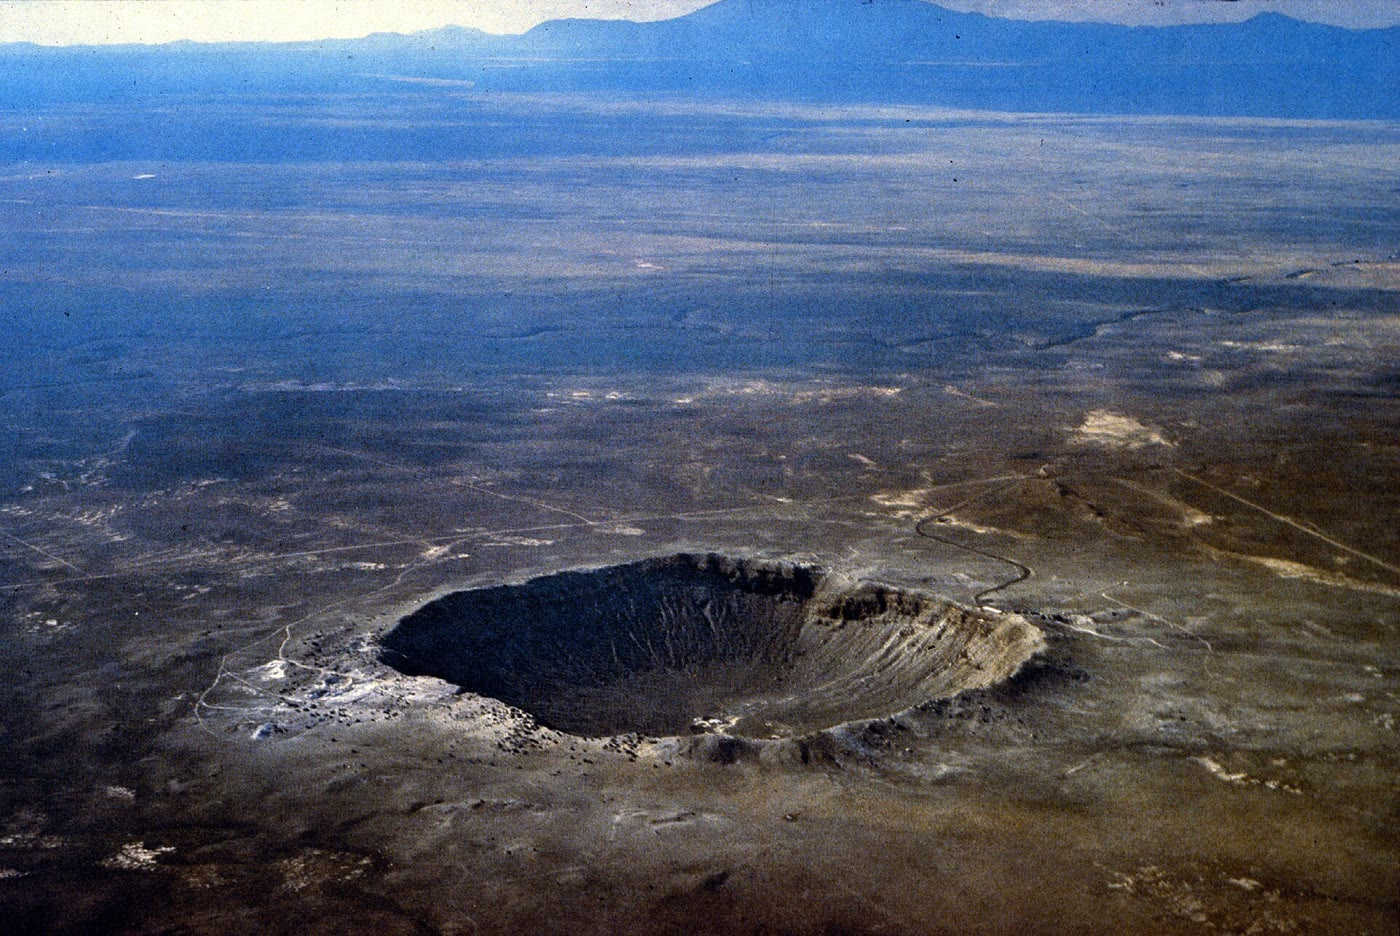
\includegraphics[width=0.66\linewidth]{images/book5/b3-barringer-crater.jpg}
\par\smallskip{\small فوهة بارينجر النيزكية، أريزونا، وهي فوهة بسيطة
قطرها \qty{1.2}{km}، تكوّنت قبل نحو 50,000 سنة بفعل نيزك حديدي
قطره نحو \qty{30}{m}؛ تعلو الحافّةُ الهضبةَ، وينتشر حولها غطاءُ
المقذوفات. صورة جوّية، \mbox{\textdir TLT USGS/D.~Roddy}، ملك
عام.}\label{fig:b3:planetary-interiors-surfaces:barringer}
\end{omfigure}
% ledger: photo:b3-barringer, french:barringer

يستغرق حفرُ فوهة قطرها \qty{1}{km} نحو ستّ ثوانٍ،
وحفرُ فوهة قطرها \qty{200}{km} نحو دقيقة ونصف. ويتوقّف حجم الفوهة
التي يُحدثها الاصطدام على طاقة القذيفة وعلى الجاذبية وعلى
مقاومة الصخر؛ والقوانين التي تربطها تُضبط على التجارب والتفجيرات
في صورة جداءات لزمرٍ عديمة البعد، ونُسلّم بها هنا. وجوهرها
يكمن في توازن الطاقات.
% ledger: french:transient

\begin{proposition}[قانون القياس في نظام الجاذبية]\label{prop:b3:planetary-interiors-surfaces:scaling}
إذا رفعت نسبةٌ ثابتة من طاقة الاصطدام $E$ الصخرَ المحفور ذا
الكثافة $\rho$ في مواجهة الجاذبية $g$، فإنّ قطر الفوهة ينمو كما يلي:
\[
  D \propto \left(\frac{E}{\rho g}\right)^{1/4} .
\]
\end{proposition}

\begin{proof}
يتناسب الحجم المحفور مع $D^3$، وكتلته مع $\rho D^3$، ويُرفع
بارتفاع من رتبة $D$: فالشغل من رتبة $\rho g D^4$، وهو
متناسب مع $E$.
\end{proof}

يذهب جزء من الطاقة إلى الحرارة وانصهار الصخر وتكسيره، لذلك
تقع القوانين الحقيقية بين هذا القانون وقواعد أبسط منه: فجدول يُستشهد به كثيرًا
للأرض يجعل عرض الفوهة عشرين ضعفًا من عرض قذيفتها الحجرية.
وتحدّد الجاذبية أيضًا الحدّ الذي تكفّ عنده الفوهة عن أن تكون بسيطة.
تنهار جدران \omterm{def:b3:planetary-interiors-surfaces:crater-morphology}{الفوهة العابرة} حين يتجاوز وزن الصخر الذي تحمله،
المقدَّر بمرتبة $\rho g D/3$، مقاومةَ الصخر، فيتناسب قطر الانتقال
عكسيًا مع $1/g$: نحو \qty{4}{km} في الصخر البلوري
و\qty{2}{km} في الرواسب على الأرض، ونحو \qty{20}{km} على
القمر، حيث الجاذبية أضعف ست مرات.
% ledger: french:table21, french:transition, planet:Earth.gravity, planet:Moon.gravity

\section{التأريخ بالفوهات}\label{sec:b3:planetary-interiors-surfaces:dating}

يكتسب السطح المتروك وحده الفوهات بالمعدّل الذي تصطدم به
الأجرام. ويُؤرَّخ السطح بعدّها، بشرط معرفة المعدّل، وأن تكون الفوهات
للسطح نفسه، لا لما يقع تحته،
ولا للحطام المقذوف من جارٍ له.

\begin{definition}[توزيع حجم الفوهات وتواترها]\label{def:b3:planetary-interiors-surfaces:sfd}
\emph{توزيع حجم الفوهات وتواترها}\index{توزيع حجم الفوهات وتواترها} لسطح ما هو العدد $N(D)$
للفوهات التي يبلغ قطرها $D$ على الأقل في وحدة المساحة،
بوصفه دالةً في $D$ (التوزيع التراكمي)، أو الأعداد المحسوبة في فئات من القطر،
تكون كل فئة عادةً أوسع من سابقتها بمقدار $\sqrt2$ مرة
(التوزيع التفاضلي).
\end{definition}

\begin{definition}[التأريخ بالفوهات؛ دالة إنتاج الفوهات ودالة كرونولوجيا الفوهات؛ كثافة توازن الفوهات]\label{def:b3:planetary-interiors-surfaces:crater-dating}
\emph{التأريخ بالفوهات}\index{التأريخ بالفوهات} هو تعيين عمر السطح
من كثافة فوهاته. وتُسمّى \emph{دالة إنتاج الفوهات}\index{دالة إنتاج الفوهات} الشكلَ
الذي يتّخذه
توزيع حجم الفوهات التي يكتسبها السطح، $F(D) =
N(D)/N(\qty{1}{km})$، ويُفترض ثبات ذلك في كل عمر. وتُسمّى
\emph{دالة كرونولوجيا الفوهات}\index{دالة كرونولوجيا الفوهات} $N_1(T)$ هو عدد الفوهات
التي يبلغ قطرها \qty{1}{km} فأكثر في وحدة المساحة المتراكمة
خلال زمن $T$. ويكون السطح عند \emph{كثافة توازن الفوهات}\index{كثافة توازن الفوهات}
لفوهات حجم معيّن، حين
تمحو كل فوهة جديدة، في المتوسط، بقدر ما تضيف من فوهات قديمة:
فلا يعود عددها يزداد.
\end{definition}

يُستنتج العمر النموذجي لسطح من عدٍّ واحد: فالعدد $N(D)$ المقاس عند أيّ $D$
يعطي $N_1 = N(D)/F(D)$، ويكون $T$ حلًّا للمعادلة $N_1(T) = N_1$. وتُسمّى الخطوط
$N(D) = N_1(T)F(D)$ عند $T$ ثابتًا إيزوكرونات. وبالنسبة إلى المرّيخ، فإنّ دالة الإنتاج
المستعملة على نطاق واسع هي كثيرةُ حدود من الدرجة~11 في $\log_{10}D$، ودالةُ
كرونولوجيا الفوهات لها الصيغة الآتية:
\[
  N_1(T) = a\left(e^{bT} - 1\right) + cT , \qquad
  a = \qty{3.22e-14}{km^{-2}}, \ b = \qty{6.93}{Ga^{-1}}, \
  c = \qty{4.875e-4}{km^{-2}.Ga^{-1}} ,
\]
خطّيةٌ خلال آخر ثلاثة مليارات سنة، وأسّيةٌ بحدّة فيما قبل ذلك. وتأخذ دالة
القمر الشكلَ نفسه، مع $a = \num{5.44e-14}$ و$c =
\num{8.38e-4}$. ضُبطت على أعمار مواقع هبوط
أبولو ولونا؛ أما دالة المرّيخ فهي دالة القمر مضروبةً في تقدير لنسبة
معدّلَي تشكّل الفوهات على المرّيخ وعلى القمر.
% ledger: craterstats:mars-pf, craterstats:mars-cf, craterstats:moon-cf, marchi:neukum

\begin{omfigure}
\centering
\begin{tikzpicture}
\begin{groupplot}[group style={group size=2 by 1, horizontal sep=1.6cm},
  width=0.48\linewidth, height=0.46\linewidth,
  tick label style={font=\scriptsize}, label style={font=\small}, title style={font=\small}]
\nextgroupplot[title={إيزوكرونات المرّيخ}, xmode=log, ymode=log, xmin=0.1, xmax=100,
  ymin=1e-8, ymax=100, xlabel={قطر الفوهة $D$ \babelsublr{(\unit{km})}},
  ylabel={\mbox{\textdir TLT $N(D)$} عدد الفوهات $\geq D$ لكلّ \unit{km^2}},
  xtick={0.1,1,10,100}, xticklabels={0.1,1,10,100},
  ytick={1e-8,1e-6,1e-4,1e-2,1}]
\addplot[thick, black!50, dashed] table[x=D, y=eq] {figdata/out/bachelor-3-crater_sfd-iso.dat};
\addplot[omDef] table[x=D, y=N_0.1] {figdata/out/bachelor-3-crater_sfd-iso.dat};
\addplot[omDef] table[x=D, y=N_1] {figdata/out/bachelor-3-crater_sfd-iso.dat};
\addplot[omDef] table[x=D, y=N_3.5] {figdata/out/bachelor-3-crater_sfd-iso.dat};
\addplot[red!70!black, thick] table[x=D, y=N_4] {figdata/out/bachelor-3-crater_sfd-iso.dat};
\node[font=\tiny, omDef, anchor=north east] at (axis cs:0.75,8e-6) {0.1~Ga};
\node[font=\tiny, omDef, anchor=north east] at (axis cs:2.6,1e-5) {1~Ga};
\node[font=\tiny, omDef, anchor=north east] at (axis cs:9,3.5e-5) {3.5~Ga};
\node[font=\tiny, red!70!black, anchor=north east] at (axis cs:45,2.5e-5) {4~Ga};
\node[font=\tiny, black!60, anchor=south, rotate=-30] at (axis cs:25,3.5e-4) {التوازن};
\nextgroupplot[title={دوال كرونولوجيا الفوهات}, ymode=log, xmin=0, xmax=4.5,
  ymin=1e-5, ymax=0.3, xlabel={العمر $T$ \babelsublr{(\unit{Ga})}}, ylabel={\mbox{\textdir TLT $N_1$} لكلّ \unit{km^2}},
  legend style={font=\scriptsize, at={(0.03,0.97)}, anchor=north west}]
\addplot[thick, red!70!black] table[x=T, y=mars] {figdata/out/bachelor-3-crater_sfd-chron.dat};
\addlegendentry{المرّيخ}
\addplot[thick, black!60, dashed] table[x=T, y=moon] {figdata/out/bachelor-3-crater_sfd-chron.dat};
\addlegendentry{القمر}
\end{groupplot}
\end{tikzpicture}
\par\smallskip{\small يسارًا: إيزوكرونات المرّيخ، والكثافات التراكمية للفوهات
على أسطح عمرها 0.1 و1 و3.5 و4 مليار سنة، مع كثافة التوازن (بخط متقطّع)
التي تحدّ من كل عدّ: فعلى سطح عمره 4 مليارات سنة تكون الفوهات الأصغر من
نحو \qty{0.7}{km} في حالة التوازن، ولا تعود تسجّل العمر. ويمينًا: دالتا الكرونولوجيا
للمرّيخ والقمر، أي عدد الفوهات التي يبلغ قطرها \qty{1}{km} فأكثر
لكلّ كيلومتر مربّع مقابل
عمر
السطح.}\label{fig:b3:planetary-interiors-surfaces:sfd}
\end{omfigure}
% ledger: craterstats:mars-pf, craterstats:mars-cf, craterstats:moon-cf, craterstats:equilibrium

تتشكّل الفوهات عشوائيًا ومستقلّةً بعضها عن بعض، فالعدد
$n$ الذي يُعثر عليه على مساحة ما متغيّرٌ بواسون.

\begin{proposition}[خطأ العدّ في العمر النموذجي]\label{prop:b3:planetary-interiors-surfaces:poisson}
إذا عُدَّ $n$ من الفوهات على مساحة $A$، فإنّ الكثافة $N = n/A$ لها انحراف معياري
قدره $\sqrt n/A$، وخطأ نسبي قدره $1/\sqrt n$، وللعمر النموذجي
انحرافٌ معياري:
\[
  \sigma_T = \frac{N_1(T)}{\sqrt n\,N_1'(T)} .
\]
\end{proposition}

\begin{proof}
قيمة متغيّرة بواسون ذات متوسط $\lambda$ يساوي تباينها $\lambda$، ويُقدَّر هذا التباين بالعدد $n$.
العمر هو $T = N_1^{-1}(N_1)$؛ وبالتقريب من الرتبة الأولى $\sigma_T =
\sigma_{N_1}/N_1'(T)$، و$\sigma_{N_1} = N_1/\sqrt n$.
\end{proof}

الخطأ النسبي للعدّ وحده يبلغ عشرة بالمئة في حالة مئة
فوهة. وعلى سطح فتيّ، حيث تكون $N_1$ خطّيةً، يرث العمر هذا الخطأ:
$\sigma_T/T = 1/\sqrt n$. أمّا على سطح قديم فإنّ الدالة الحادّة تُنقص هذا الخطأ بمقدار
ستّة أضعاف عند \qty{3.8}{Ga} (\cref{exo:b3:planetary-interiors-surfaces:11})؛
فتتقيّد الأعمار النموذجية للأسطح القديمة عندئذٍ
بمعايرة الدالة نفسها. ويقيّد العدّ حدّان آخران: تتشبّع الفوهات الصغيرة،
فعلى أقدم الأسطح تبلغ الفوهات التي يقلّ قطرها عن نحو \qty{0.7}{km}
\omterm{def:b3:planetary-interiors-surfaces:crater-dating}{كثافة توازن الفوهات}، فلا تسجّل الزمن بعد ذلك. ويمكن أن يُجدَّد السطح دون أن يُمحى:
فتدفّق حممي يدفن الفوهات الصغيرة دون حواف الكبيرة يترك توزيعًا فيه انثناء،
قديمًا عند $D$ الكبيرة وفتيًّا عند $D$ الصغيرة.
ويؤرّخ هذا الانثناء \omterm{def:b3:planetary-interiors-surfaces:resurfacing}{تجديد السطح}.
% ledger: craterstats:equilibrium

\begin{definition}[تجديد السطح]\label{def:b3:planetary-interiors-surfaces:resurfacing}
\emph{تجديد السطح}\index{تجديد السطح} هو تجديدُ سطحٍ كوكبي
بالحمم أو الرواسب أو الجليد أو التشوّه، يزيل فوهاته أو يدفنها
ويُعيد ضبط ساعة الفوهات فيه.
\end{definition}

\section{البركانية والتكتونية خارج الأرض}\label{sec:b3:planetary-interiors-surfaces:volcanism}

كلّ كوكب صخري يفقد حرارته الداخلية عبر غلافه الصخري.
تفعل الأرض ذلك بصفائح متحرّكة، أمّا الكواكب الأخرى فتفعله بطريقة مختلفة.

\begin{definition}[الغطاء الراكد]\label{def:b3:planetary-interiors-surfaces:stagnant-lid}
يمتلك الكوكب \emph{الغطاء الراكد}\index{الغطاء الراكد} حين يكون غلافه الصخري
قشرةً صلبةً واحدةً لا تشارك في الحمل الحراري للوشاح
الواقع تحتها: تعبر الحرارةُ منها بالتوصيل وبالمصهور الذي يصعد
عبرها. وعلى كوكب ذي غطاء متحرّك كالأرض، يتفتّت الغلاف الصخري
إلى صفائح تعود فتغوص في الوشاح.
\end{definition}

\begin{definition}[البركانية بالأنبوب الحراري]\label{def:b3:planetary-interiors-surfaces:heat-pipe}
\emph{البركانية بالأنبوب الحراري}\index{البركانية بالأنبوب الحراري} هي فقدانُ الكوكب حرارتَه الداخلية أساسًا
بصعود المصهور عبر قنوات ضيّقة وثورانه على السطح،
حيث تبرد الحمم ويدفنها ما يليها من حمم،
فيُبنى الغلاف الصخري من أعلاه ويُحمل إلى الأسفل باردًا.
\end{definition}

\begin{omfigure}
\centering
\begin{tikzpicture}[x=0.5cm, y=0.5cm, font=\scriptsize, >=stealth]
\foreach \dx/\name in {0/{الغطاء المتحرّك}, 9.5/{الغطاء الراكد}, 19/{الأنبوب الحراري}} {
  \begin{scope}[xshift=\dx*0.5cm]
  \fill[orange!15] (0,0) rectangle (8,4);
  \node[anchor=south] at (4,5.6) {\name};
  \end{scope}}
% mobile lid: plates, ridge, slab
\fill[omDef!35] (0,4) rectangle (3.9,4.8);
\fill[omDef!35] (4.1,4) rectangle (6.2,4.8);
\fill[omDef!35] (6.2,4.8) -- (7.6,1.6) -- (6.9,1.4) -- (5.5,4.0) -- cycle;
\fill[omDef!35] (6.55,4) rectangle (8,4.8);
\draw[->, thick] (3.6,5.1) -- (1.6,5.1); \draw[->, thick] (4.4,5.1) -- (6.0,5.1);
\draw[->, red!70!black] (4,1.0) -- (4,3.6);
\draw[black!60, ->] (2.0,3.4) arc (90:270:1.0 and 1.2);
\node[anchor=north] at (4,-0.2) {الصفائح تغوص};
% stagnant lid
\begin{scope}[xshift=4.75cm]
\fill[omDef!35] (0,3.2) rectangle (8,4.8);
\draw[black!60, ->] (2.4,3.0) arc (90:270:1.2 and 1.2);
\draw[black!60, ->] (5.6,0.6) arc (-90:90:1.2 and 1.2);
\fill[red!70!black] (3.9,3.2) rectangle (4.1,4.8);
\fill[red!70!black] (3.0,4.8) -- (4,5.4) -- (5.0,4.8) -- cycle;
\node[anchor=north] at (4,-0.2) {قشرة واحدة سميكة};
\end{scope}
% heat pipe
\begin{scope}[xshift=9.5cm]
\fill[omDef!35] (0,1.0) rectangle (8,4.8);
\foreach \x in {1.5,4,6.5} {\fill[red!70!black] (\x-0.1,1.0) rectangle (\x+0.1,4.8);
  \fill[red!70!black] (\x-0.6,4.8) -- (\x,5.2) -- (\x+0.6,4.8) -- cycle;}
\draw[->, thick] (2.75,4.3) -- (2.75,1.6); \draw[->, thick] (5.25,4.3) -- (5.25,1.6);
\node[anchor=north] at (4,-0.2) {حمم مدفونة، غطاء بارد};
\end{scope}
\end{tikzpicture}
\par\smallskip{\small ثلاث طرق لفقد الحرارة (رسم تخطيطي). يسارًا: غطاء
متحرّك، صفائح تتكوّن عند الظهرات وتغوص عند الخنادق، كما هي الحال على
الأرض. وفي الوسط: \omterm{def:b3:planetary-interiors-surfaces:stagnant-lid}{غطاء راكد}، قشرة صلبة واحدة فوق الوشاح الحامل،
يعبرها مصهور عدد قليل من البراكين طويلة العمر. ويمينًا: الأنابيب الحرارية،
مصهور يصعد عبر غلاف صخري سميك وبارد في قنوات ضيّقة،
فتدفنها حمم لاحقة وتُحمل
إلى الأسفل.}\label{fig:b3:planetary-interiors-surfaces:lids}
\end{omfigure}

يمتلك المريخ \omterm{def:b3:planetary-interiors-surfaces:stagnant-lid}{غطاءً راكدًا}. ومن دون صفائح تحمل حممه بعيدًا عن
مصادرها، نمت براكينه في موضعها زمنًا طويلًا فوق انتفاخ
تارسيس. يُعرف أوليمبوس مونس بأنّه أكبر بركان معروف في النظام الشمسي، ويرتفع
\qty{27}{km} على قاعدة يزيد عرضها على \qty{600}{km}، تحيط بها
جرف صدعي يبلغ ارتفاعه \qty{6}{km}؛ ويبلغ عرض كلٍّ من براكين تارسيس مونتيس الثلاثة المجاورة من 350
إلى \qty{400}{km} عرضًا. يثني حملٌ بهذا الحجم الغلاف الصخري، ويقيس عرض
الخندق الذي يحفره، كما على الأرض، السماكةَ المرنة
\omterm{def:b3:planetary-interiors-surfaces:stagnant-lid}{للغطاء الراكد}.
% ledger: nasa:olympus-mons

\begin{omfigure}
\centering
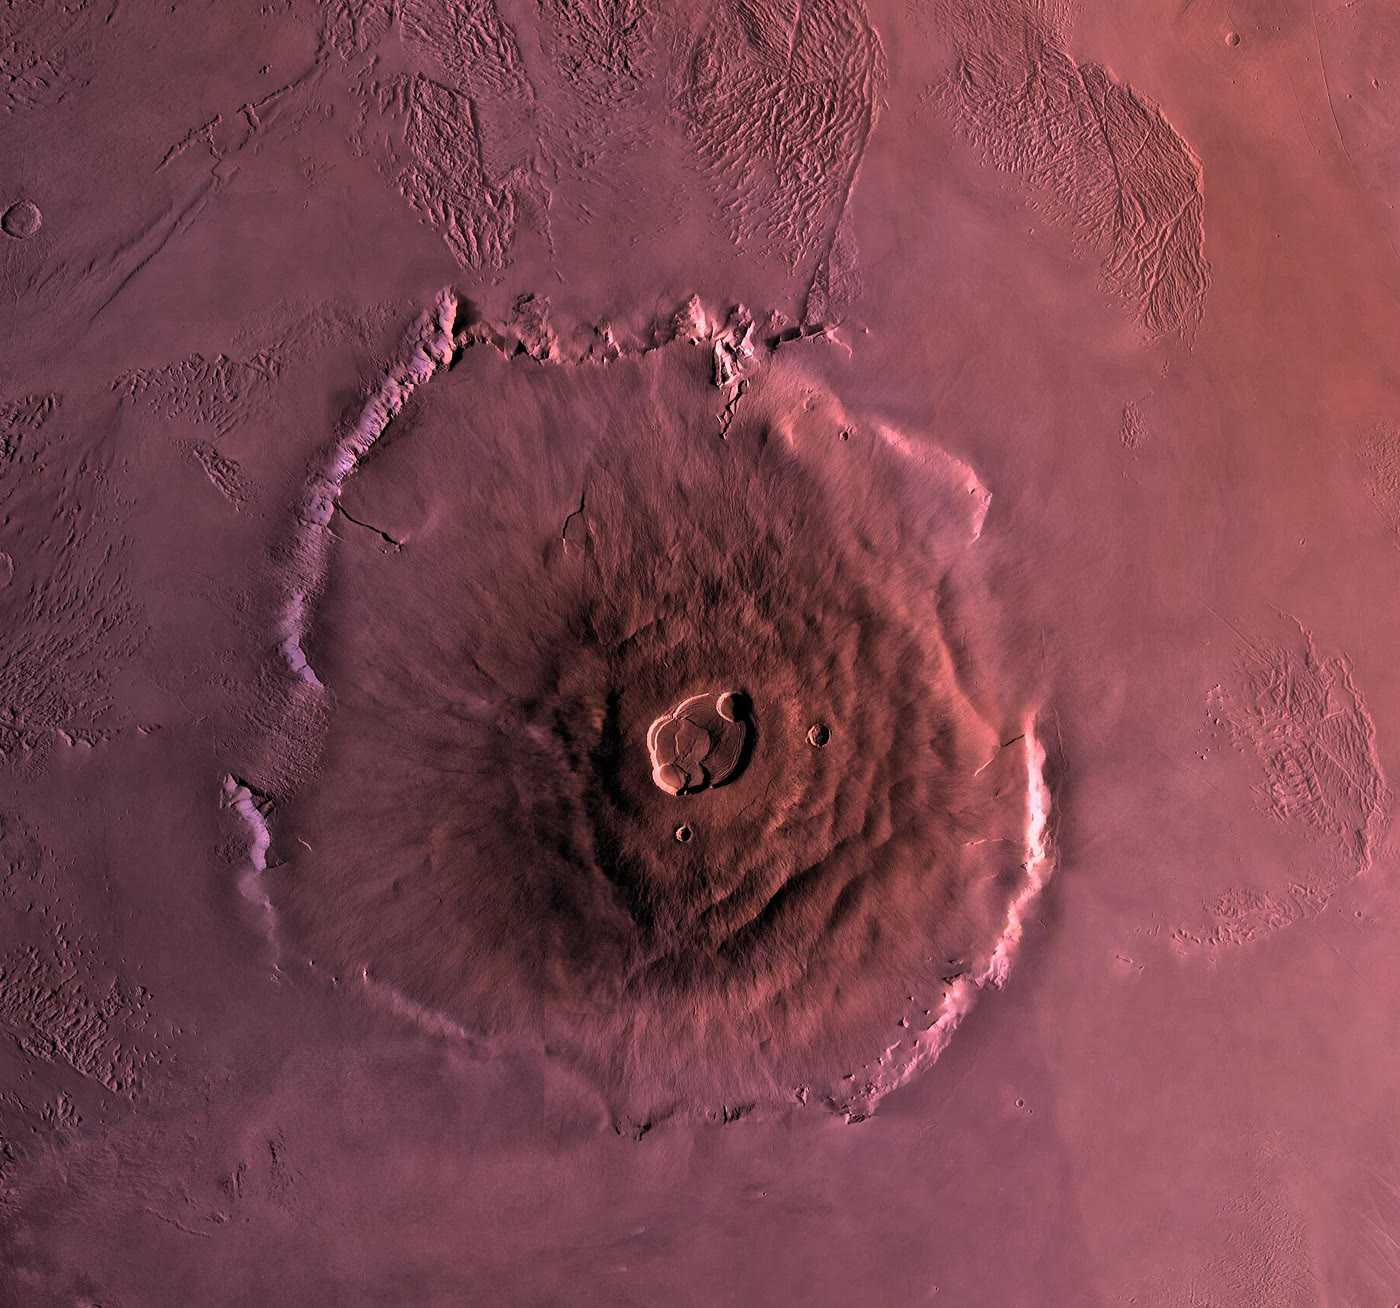
\includegraphics[width=0.48\linewidth]{images/book5/b3-olympus-mons.jpg}
\par\smallskip{\small أوليمبوس مونس على المريخ، فسيفساء من صور
مركبات فايكنغ المدارية: الكالديرات القمّية في الوسط، وسفوح تدفّقات الحمم
والجرف الصدعي المنحدر الذي يحيط بالقاعدة، ويبلغ عرض بعضها نحو \qty{600}{km}.
\mbox{\textdir TLT NASA/JPL/USGS}، ملك عام.}\label{fig:b3:planetary-interiors-surfaces:olympus}
\end{omfigure}
% ledger: photo:b3-olympus-mons, nasa:olympus-mons

الزهرة، المماثلة للأرض في الحجم، تملك بفارق كبير أقلّ فوهات الاصطدام من
أيّ كوكب صخري آخر ما عدا الأرض.
قد يكون متوسط عمر ملامح سطحها نحو 150 مليون سنة، مع رقع أقدم بينها:
البركانية والتشوّه جدّدا معظم سطحها، ربما على مراحل متفرّقة
عبر زمن طويل، وربما بوتيرة أسرع. ولدى الزهرة آلاف البراكين ولا أثر
لصفائح متحرّكة.
% ledger: nasa:venus-surface, planet:Venus.diameter, planet:Earth.diameter

آيو، أقرب أقمار المشتري الكبيرة إليه، تفقد أكثر من
\qty{2.5}{W.m^{-2}} عبر سطحها، أي نحو 27 ضعف المتوسط الأرضي
البالغ \qty{0.092}{W.m^{-2}}. وحرارتها ليست حرارة النشاط الإشعاعي، بل
تولّدها المدّات.
% ledger: veeder:io-heat, dd10:split

\begin{definition}[التسخين المدّي]\label{def:b3:planetary-interiors-surfaces:tidal-heating}
\emph{التسخين المدّي}\index{التسخين المدّي} هو الحرارة المتولّدة داخل
جرم بفعل احتكاك التشوّه الذي يفرضه عليه مدّ متغيّر.
يرى القمر الذي يدور بالتزامن على مدار شديد الاستطالة مدّ كوكبه
يتغيّر في شدّته ويتأرجح ذهابًا وإيابًا خلال كلّ دورة.
\end{definition}

\begin{proposition}[استطاعة المدّ لقمر متزامن]\label{prop:b3:planetary-interiors-surfaces:tidal-power}
يبدّد قمر نصف قطره $R$ يدور بالتزامن، على مدار متوسّط حركته
$n$ وذو لا مركزية صغيرة $e$، الاستطاعة
\[
  \dot E = \frac{21}{2}\,\frac{k_2}{Q}\,\frac{(nR)^5}{G}\,e^2 ,
\]
حيث $Q$ عامل الجودة المدّية للقمر، بحيث يقيس $k_2/Q$
الجزء من التشوّه المدّي الذي يفقد على هيئة حرارة.
\end{proposition}

يُقبل الاقتراح. والمدّات التي تبدّد الطاقة تُدوّر المدار أيضًا،
لكنّ مدار آيو يبقى بيضاويًا، بلا انحراف يتجاوز 0.004، لأنّ
جذبات أوروبا وغانيميد المتوقَّتة بدقّة تضطرب مداره، إذ
تقف دوراتهما المدارية البالغة 1.77 و3.55 و\num{7.15}~يومًا عند
نسبة 1:2:4 تقريبًا تمامًا (انظر \cref{exo:b3:planetary-interiors-surfaces:8}). ويرتفع سطحه
وينخفض بمقدار يبلغ \qty{100}{m} في كلّ دورة. وتغطّي البراكين
آيو بالحمم أسرع مما تتكوّن عليه الفوهات؛ ومن النماذج التي تفسّر كيف يتسرّب
حرارته عبر \omterm{def:b3:planetary-interiors-surfaces:heat-pipe}{البركانية بالأنبوب الحراري}، وهو نموذج يُبقي على غلاف صخري سميك
وبارد تحت سطحه المتّقد.
% ledger: nasa:galilean-orbits, beuthe:tidal-power, nasa:io-orbit, nasa:io-facts

\begin{definition}[المحيط تحت السطحي]\label{def:b3:planetary-interiors-surfaces:ocean-world}
\emph{المحيط تحت السطحي}\index{المحيط تحت السطحي} طبقة عالمية من
الماء السائل تقع تحت الغطاء الجليدي لقمر أو كوكب قزم، وتبقى سائلة بفعل
الحرارة المدّية والحرارة المشعّة.
\end{definition}

\begin{definition}[البركانية الجليدية]\label{def:b3:planetary-interiors-surfaces:cryovolcanism}
\emph{البركانية الجليدية}\index{البركانية الجليدية} هي اندفاع الماء والمحاليل
الملحية أو غيرها من السوائل والأبخرة المتطايرة، بدلًا من الصخر المنصهر، إلى
السطح الجليدي لقمر أو كوكب قزم.
\end{definition}

قُدّر غطاء أوروبا الجليدي، بقياس مقياس الإشعاع الميكروي لمركبة جونو
الفضائية في المنطقة التي حلّقت فوقها، بمتوسّط سماكة نحو \qty{29}{km}؛
ويقع تحته محيط مالح يحتوي ضعف ما تحويه
محيطات الأرض كلّها من ماء. وعلى قمر زحل إنسيلادوس، الذي لا يتجاوز عرضه
نحو \qty{500}{km}، وجدت مركبة كاسيني الفضائية عام 2005 نفاثات من حبيبات الجليد والغاز
تنطلق من شقوق دافئة قرب القطب الجنوبي بسرعة نحو
\qty{400}{m.s^{-1}}. وأظهرت جاذبيته واهتزاز دورانه أنّ
النفاثات تستمدّ من محيط عالمي يقع تحت غطاء جليدي يبلغ متوسّط سماكته من 20 إلى
\qty{25}{km}، وربما لا يتجاوز من 1 إلى \qty{5}{km} عند
القطب الجنوبي.
% ledger: jpl:europa-shell, nasa:europa-ocean, nasa:enceladus

\section{اللبّات الكبيرة والصغيرة}\label{sec:b3:planetary-interiors-surfaces:cores}

تشكّل اللبّات الأربعة المقاسة مجموعة غريبة. فبالنسبة إلى نصف القطر، يبلغ
لبّ الأرض 0.55 من المسافة إلى السطح، ولبّ المرّيخ 0.54؛ ولبّ القمر
0.19؛ ولبّ عطارد 0.82. ويفرز التمايز، في مجلد السنة الثانية،
المعدن عن السيليكات داخل كلّ جرم، لكنّه لا يستطيع أن يجعل نسب المعدن
مختلفة إلى هذا الحدّ. أمّا الاصطدامات الهائلة فتستطيع ذلك. يُعتقد أنّ القمر تكوّن
من حطام تصادم بين جرم بحجم المرّيخ والأرض
الفتيّة قبل نحو 4.5 مليار سنة، إذ انضمّ معدن الجرم المصطدم
إلى لبّ الأرض، وتجمّع في القمر في معظمه صخر الوشاح، ومن هنا
لبّه الصغير. وربما أزالت اصطدامات مماثلة جزءًا كبيرًا من وشاح السيليكات
لعطارد، فصار كوكبًا غنيًّا بالحديد يملأ لبّه معظمه.
وتسجّل اللبّات، كما تسجّل الفوهات، تاريخًا من الاصطدامات.
% ledger: data:prem, jpl:insight-interior, nasa:moon-core, agu:mercury-core, french:giant-impacts

\section{التمارين}

\begin{exercise}[$\star$]\label{exo:b3:planetary-interiors-surfaces:1}
لعطارد متوسّط كثافة يبلغ \qty{5429}{kg.m^{-3}}، وعامل عزم القصور الذاتي
يبلغ 0.35، ونصف قطر يبلغ \qty{2440}{km}. باستخدام نموذج من طبقتين ووشاح
كثافته \qty{3300}{kg.m^{-3}}، احسب نصف القطر النسبي للبّ،
ونصف قطره بالكيلومترات، وكثافته.
\end{exercise}

\begin{exercise}[$\star$]\label{exo:b3:planetary-interiors-surfaces:2}
قذيفة حجرية قطرها \qty{50}{m}، وكثافتها \qty{3500}{kg.m^{-3}}،
تصطدم بالأرض عموديًّا بسرعة \qty{20}{km.s^{-1}}. احسب كتلتها وطاقتها الحركية،
بالجول وبالميغاطن من المتفجّرات
($\qty{1}{Mt} = \qty{4.2e15}{J}$). ما قطر الفوهة الذي تعطيه قاعدة
عشرين ضعف قطر القذيفة؟
\end{exercise}

\begin{exercise}[$\star$]\label{exo:b3:planetary-interiors-surfaces:3}
على سهل مرّيخي مساحته \qty{100000}{km^2}، تُعدّ 120 فوهة قطرها
\qty{1}{km} فأكثر. احسب $N_1$، وخطأه النسبي، والعمر النموذجي للسهل
مع خطئه.
\end{exercise}

\begin{exercise}[$\star$]\label{exo:b3:planetary-interiors-surfaces:4}
آيو، ونصف قطرها \qty{1821.5}{km}، تفقد \qty{2.5}{W.m^{-2}}. احسب فقدها الحراري
الكلّي، وقارنه بالفقد الأرضي البالغ \qty{47}{TW}، كليًّا
ولكلّ متر مربّع (\qty{0.092}{W.m^{-2}}).
\end{exercise}

\begin{exercise}[$\star\star$]\label{exo:b3:planetary-interiors-surfaces:5}
للمرّيخ كتلة مقدارها \qty{6.417e23}{kg} ونصف قطر مقداره \qty{3389.5}{km}.
(أ)~احسب كثافته المتوسّطة، وجاذبيته السطحية، و$\rho gR$.
(ب)~بمعاملته كرة متجانسة غير قابلة للانضغاط صلابتها
\qty{67}{GPa}، احسب \omterm{def:b3:planetary-interiors-surfaces:love-number}{عدد لوف} $k_2$. (ج)~القيمة المقاسة هي
$0.153 \pm 0.017$. ماذا تقول المقارنة؟
\end{exercise}

\begin{exercise}[$\star\star$]\label{exo:b3:planetary-interiors-surfaces:6}
على الأرض ($g = \qty{9.8}{m.s^{-2}}$) يحدث الانتقال من \omterm{def:b3:planetary-interiors-surfaces:crater-morphology}{الفوهة البسيطة} إلى المعقّدة
يقع تقريبًا عند \qty{4}{km} في الصخر البلّوري و\qty{2}{km} في
الرواسب. (أ)~بافتراض أنّ قطر الانتقال يتناسب مع $1/g$،
توقّعه على القمر ($g = \qty{1.62}{m.s^{-2}}$) وعلى المرّيخ
وعطارد ($g = \qty{3.7}{m.s^{-2}}$)؛ قارنه بالقيمة \qty{20}{km}
المرصودة على القمر. (ب)~إذا بدأ الانهيار حين يتجاوز $\rho gD/3$
مقاومةَ الصخر $Y$، فما المقاومة التي يعطيها الانتقال البلّوري
على الأرض من أجل $\rho = \qty{2600}{kg.m^{-3}}$؟
\end{exercise}

\begin{exercise}[$\star\star$]\label{exo:b3:planetary-interiors-surfaces:7}
يحمل سطحٌ ما $\num{2.0e-3}$ فوهةً قطرها \qty{1}{km} فأكثر لكلّ
كيلومتر مربّع. أوجِد عمره النموذجي \omterm{def:b3:planetary-interiors-surfaces:crater-dating}{بدالة كرونولوجيا الفوهات} الخاصّة بالمرّيخ،
بحلّ المعادلة عدديًّا. وما العمر الذي كانت ستعطيه دالة القمر،
ولماذا لا يجوز تبادل الدالتين؟
\end{exercise}

\begin{exercise}[$\star\star$]\label{exo:b3:planetary-interiors-surfaces:8}
الدورات المدارية لآيو وأوروبا وغانيميد هي 1.769138، 3.551181
و\num{7.154553}~يومًا. (أ)~احسب نسب الدورات المتعاقبة.
(ب)~احسب $1/P_I - 3/P_E + 2/P_G$ وعلّق. (ج)~لماذا يمكن للرنينات
أن تحفظ اللامركزيةَ التي كانت المدّات ستزيلها لولاها؟
\end{exercise}

\begin{exercise}[$\star\star$]\label{exo:b3:planetary-interiors-surfaces:9}
يدور آيو حول المشتري في \num{1.769138}~يومًا بلامركزية 0.004.
احسب الاستطاعة التي تعطيها القضيّة المتعلّقة باستطاعة المدّ لكلّ وحدة من $k_2/Q$،
وقيمة $k_2/Q$ التي تكفي لتغطية فقد حرارة آيو
المذكور في \cref{exo:b3:planetary-interiors-surfaces:4}.
\end{exercise}

\begin{exercise}[$\star\star\star$]\label{exo:b3:planetary-interiors-surfaces:10}
من أجل القمر، $\bar\rho = \qty{3340}{kg.m^{-3}}$ و$C = 0.394$.
(أ)~بيّن أنّه في نموذج الطبقتين $\mathrm dx^2/\mathrm dC =
\tfrac52\bar\rho/(\bar\rho - \rho_m)$ عندما تكون $\rho_m$ ثابتة. (ب)~مع
كثافة الوشاح التي تعطي لبًّا نصف قطره النسبي $x = 0.19$، وهي \qty{3288}{kg.m^{-3}}،
ما قيمة $x$ و$\rho_c$ عندما يكون $C = 0.395$، وعندما يكون $C = 0.393$؟
(ج)~ماذا تقول هذه النتيجة عن تعيين لبٍّ صغير بواسطة
عامل عزم القصور الذاتي؟
\end{exercise}

\begin{exercise}[$\star\star\star$]\label{exo:b3:planetary-interiors-surfaces:11}
(أ)~من أجل 100 فوهة، احسب خطأ العدّ في العمر النموذجي لسطح
مرّيخي عمره \qty{1.0}{Ga} ولآخر عمره \qty{3.8}{Ga}.
(ب)~بيّن أنّه على الجزء الخطّي من دالة الكرونولوجيا $\sigma_T/T =
1/\sqrt n$. (ج)~لماذا تبقى أعمار الأسطح القديمة غير مؤكَّدة إذن؟
\end{exercise}

\begin{exercise}[$\star\star\star$]\label{exo:b3:planetary-interiors-surfaces:12}
أوروبا، ونصف قطره \qty{1560.8}{km}، يدور في \num{3.551181}~يومًا بلامركزية
0.009. (أ)~إذا بدّدت أوروبا المدّات بالقيمة $k_2/Q$ نفسها التي لآيو،
فما الكسر من استطاعة المدّ لآيو الذي كانت ستولّده، وما التدفّق الحراري؟
(ب)~لماذا يكون الافتراض مشكوكًا فيه لقمرٍ له محيط تحت جليده؟
\end{exercise}

\section{مسألة: سهلان على المرّيخ}

\begin{problem}[{مسألة نهاية الأسبوع --- لبّ المرّيخ وعمرا سهلين
حمميّين مختلقين}]
\label{pb:b3:planetary-interiors-surfaces:1}
للمرّيخ كتلة مقدارها \qty{6.4169e23}{kg}، ونصف قطر مقداره \qty{3389.5}{km}،
وعامل عزم القصور الذاتي 0.366. يقع سهلان مختلقان، هما A و B، على
أقاليمه البركانية؛ وقد عُدّت فوهاتهما على صور في فئات
عرض كلّ منها $\sqrt2$.

\medskip\noindent\textbf{الجزء الأول --- اللبّ.}
\begin{enumerate}
\item احسب متوسّط كثافة المرّيخ.
\item باستخدام نموذج الطبقتين ووشاح كثافته \qty{3500}{kg.m^{-3}}، احسب
  نصف القطر النسبي للّبّ، ونصف قطره بالكيلومترات،
  وكثافته.
\item قاست المهمّة إنسايت نصف قطر لبٍّ قدره \qty{1830}{km}. ما كثافتا الوشاح واللبّ
  اللتان يقتضيهما نموذج الطبقتين إذن؟
\item قارن كثافة هذا اللبّ بكثافة اللبّ الخارجي للأرض
  قرب قمّته مباشرة، \qty{9900}{kg.m^{-3}} في نموذج الأرض المرجعي،
  وبيّن لماذا تُتوقَّع قيمةٌ أدنى للمرّيخ، وما الذي يوحي به
  أيضًا.
\item \omterm{def:b3:planetary-interiors-surfaces:love-number}{عدد لوف} للكرة المتجانسة للمرّيخ عند صلابة مقدارها
  \qty{67}{GPa} يساوي 0.109، والقيمة المقيسة 0.153. أيّ الرصدين جاء
  أوّلًا، وما الذي قاله مسبقًا عن اللبّ؟
\item يتراوح سمك قشرة المرّيخ بين 20 و\qty{37}{km}. ما الكسر من
  حجم الكوكب الذي تحتويه؟ وهل كان من الصواب إهمالها؟
\end{enumerate}

\medskip\noindent\textbf{الجزء الثاني --- العدّ على السهل A.} السهل A
يغطي \qty{80000}{km^2}. فوهاته، حسب فئات القطر \babelsublr{(km)}:
\begin{center}
\small
\begin{tabular}{lccccccccc}
\hline
الفئة & \mbox{\textdir TLT 1--1.41} & \mbox{\textdir TLT 1.41--2} & \mbox{\textdir TLT 2--2.83} & \mbox{\textdir TLT 2.83--4} & \mbox{\textdir TLT 4--5.66} & \mbox{\textdir TLT 5.66--8} & \mbox{\textdir TLT 8--11.3} & \mbox{\textdir TLT 11.3--16} & \mbox{\textdir TLT 16--22.6} \\
\hline
السهل A & 38 & 6 & 5 & 3 & 0 & 0 & 0 & 1 & 1 \\
السهل B & 48 & 8 & 31 & 12 & 7 & 2 & 0 & 2 & 2 \\
\hline
\end{tabular}
\end{center}
\begin{enumerate}[resume]
\item احسب العدّ التراكمي للسهل A، ابتداءً من \qty{1}{km}.
\item احسب $N(\qty{1}{km})$ لكلّ كيلومتر مربّع وانحرافه
  المعياري.
\item تعطي دالة الإنتاج $F(\qty{2}{km}) = 0.147$
  و$F(\qty{1.41}{km}) = 0.355$. هل تتّسق أعداد الفوهات عند 1.41 و\qty{2}{km}
  مع شكل دالة الإنتاج؟
\item هل السهل A قريب بأيّ قدر من \omterm{def:b3:planetary-interiors-surfaces:crater-dating}{كثافة توازن الفوهات}،
  \qty{0.072}{km^{-2}} عند \qty{1}{km}؟
\item لماذا اختيرت الفئات بعرض $\sqrt2$؟
\item تُستبعد عناقيد الفوهات الصغيرة وسلاسلها من العدّ. لماذا؟
\end{enumerate}

\medskip\noindent\textbf{الجزء الثالث --- الأعمار النموذجية.} استخدم \omterm{def:b3:planetary-interiors-surfaces:crater-dating}{دالة كرونولوجيا
الفوهات} الخاصة بالمريخ.
\begin{enumerate}[resume]
\item احسب العمر النموذجي للسهل A. تحقّق من أنّ الحدّ الأُسّي
  يمكن إهماله.
\item احسب خطأ العدّ الخاص به.
\item أيّ عمر كان سيعطيه التأريخ القمري؟
\item يغطّي السهل B مساحة \qty{120000}{km^2}. باستخدام فوهاته التي قطرها \qty{2}{km}
  فأكثر، احسب $N(\qty{2}{km})$، ثم $N_1$، ثم عمره النموذجي، بحلّ
  المعادلة عدديًّا.
\item احسب خطأ العدّ لذلك العمر.
\item قارن الأخطاء النسبية للعمرين، وفسّر
  الفرق بينهما.
\end{enumerate}

\medskip\noindent\textbf{الجزء الرابع --- الفوهات المدفونة في السهل B.}
\begin{enumerate}[resume]
\item كم فوهة يُفترض أن يحملها السهل B، بقطر بين 1 و\qty{2}{km}، إذا كان سطحه كلّه بعمر السؤال~16؟
  وكم فوهة يحملها فعلًا؟
\item افترض أنّ الحمم دفنت كلّ فوهة أصغر من \qty{2}{km} عند زمن $T_r$
  وأبقت على الفوهات الأكبر. احسب $T_r$ من الفوهات
  التي قطرها \num{1}--\qty{2}{km}.
\item احسب خطأ العدّ للزمن $T_r$.
\item افترض أنّ \omterm{def:b3:planetary-interiors-surfaces:crater-morphology}{الفوهة البسيطة} الحديثة على المريخ عمقها خُمس عرضها
  (افتراض في هذه المسألة). ما سُمك الحمم اللازم لدفن
  فوهة قطرها \qty{2}{km}، ولماذا ما زالت الفوهات الأكبر ظاهرة؟
\item هل يمكن أن تنتمي حمم السهل B وحمم السهل A إلى حدث
  بركاني واحد؟
\item أعطِ العمر النموذجي للسهل A بالمليارات من السنين، إلى
  رقمين معنويّين.
\end{enumerate}
\end{problem}
% ledger: nasa:mars, jpl:insight-interior, yoder:mars-k2, data:prem, craterstats:mars-pf, craterstats:mars-cf, craterstats:moon-cf, craterstats:equilibrium
